\newpage
\section{Physically Based Rendering}
\label{sec:pbr}
\hspace{\parindent}
It needs to be stated that the engine utilizes PBR - physically based rendering. It is a rendering technique simulating the behavior of real light rays, which can create spectacularly realistic images. Physically based rendering used to be a too complex algorithm to use in real time, like it is used in TSEngine, however, with the growing capabilities of the computers for the last decades it has become more common for real time usage of the technique in real time applications, for example in computer games.
\begin{figure}[H]
    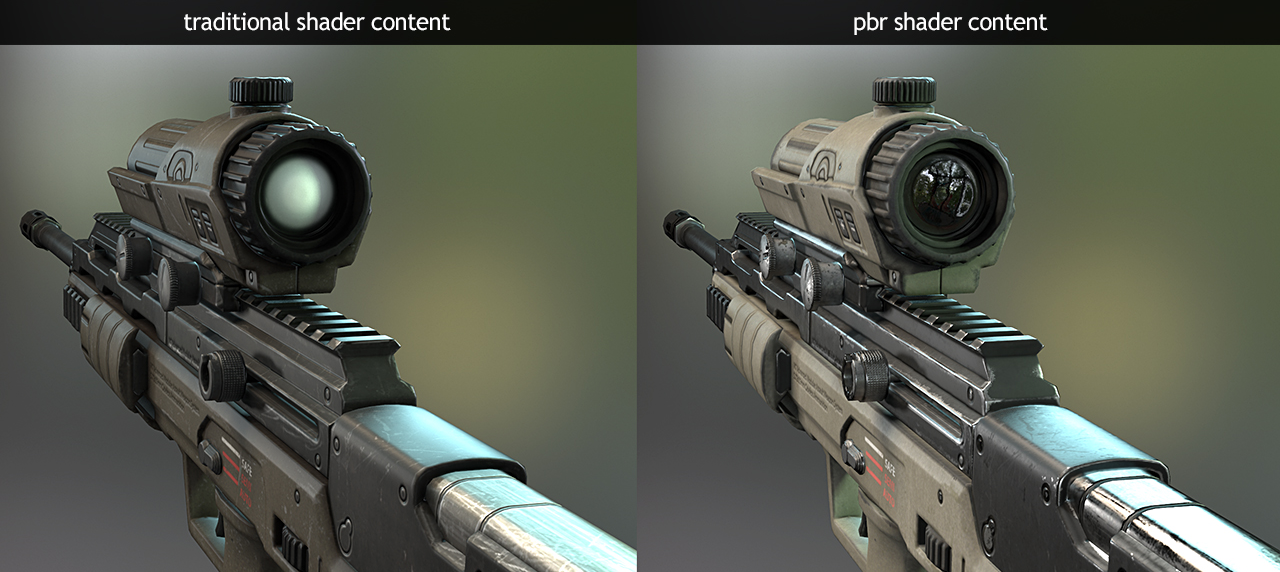
\includegraphics[width=\linewidth]{PBR-Example-Meta3DStudios.png}
    \caption{Image showing advantages of PBR from META 3D Studios \cite{pbrExample} }
\end{figure}
Many of the nowadays implementations of the algorithm, are based on the paper from 2012, Physically Based Shading at Disney by Brent Burley, Walt Disney Animation Studios. This work accumulates much of the knowledge from studies made on PBR since 1960s and builds on it. Its main defining feature is the usage of the BRDF - bidirectional reflective distribution function, which takes the incoming ($\omega i$) and outgoing ($\omega o$) directions, normal (n) of the surface and different parameters defining the surface's properties. TSEngine can only take the surface's roughness, albedo or metallic as a parameters and uses Cook-Torrance specular bidirectional reflective distribution function, which is defined as follows:
\begin{equation}
f_{CookTorrance}=\frac{DFG}{4(\omega_{O} \cdot n)(\omega_{i} \cdot n)}
\text{ .}
\label{EquationCookTorrance}
\end{equation}
As one can see, the function is composed of three different functions D, F and G and a normalization factor. Each of the three functions is responsible for approximating specific part of the surface's reflective properties:\\
D - Represents normal distribution function, also known as Gaussian distribution or bell curve, showing how probability is distributed. It is responsible for approximating how many of all the microfacets are aligned with the halfway vector, which is the vector halfway between the viewer and the light source. \\
\begin{equation}
NDF_{GGXTR}(n, h, \alpha) = \frac{\alpha^2}{\pi((n \cdot h)^2(\alpha^2 - 1) + 1)^2}
\text{ .}
\end{equation}
G - Geometry function is approximating how much of the surface's reflective microfacets are overshadowed by other microfacets casting shadows. The rougher the surface, the less light surface can reflect.
\begin{equation}
G_{SchlickGGX}(n, v, k) = \frac{n \cdot v}{(n \cdot v)(1 - k) + k}
\text{ ,}
\end{equation}
\begin{equation}
k_{direct} = \frac{(\alpha + 1)^2}{8}
\text{ ,}
\end{equation}
\begin{equation}
G_{SchlickSmithGGX}(n, v, l, k) = G_{sub}(n, v, k) G_{sub}(n, l, k)
\text{ .}
\end{equation}

F - Is the Fresnel equation, which describes the behavior of light waves (reflection, distortion) when they encounter a change in media. In Cook-Torrance method, it is used to approximate the ratio of surface reflection depending on the surface's angle.\\ 
%explain the ratio of surface reflection depending on the surface's angle better
\begin{equation}
F_{Schlick}(h, v, F_0) = F_0 + (1 - F_0)(1 - (h \cdot v))^5
\text{ .}
\end{equation}
Based on the book \textit{"Learn OpenGL"} \cite{learnopengl} and the article \textit{"Specular BRDF Reference"} \cite{pbrreferences}.